% ============================================================
% 2020 高教社杯全国大学生数学建模竞赛
% A题：自来水厂水质预测与评估
% ============================================================
\documentclass[12pt,a4paper]{ctexart}

% ---------- 页面设置 ----------
\usepackage[top=2.5cm, bottom=2.5cm, left=2.5cm, right=2.5cm]{geometry}
\usepackage{amsmath,amssymb}
\usepackage{graphicx}
\usepackage{booktabs}
\usepackage{tabularx}
\usepackage{caption}
\usepackage{hyperref}
\usepackage{enumitem}
\usepackage{float}
\usepackage{fancyhdr}
\setlength{\headheight}{14pt}
\setlength{\parindent}{2em}
\setlength{\parskip}{3pt}
\usepackage{xcolor}
\usepackage{listings}
\lstset{
    basicstyle=\small\ttfamily,
    numbers=left,
    numberstyle=\tiny\color{gray},
    frame=single,
    backgroundcolor=\color{gray!10},
    rulecolor=\color{gray!50},
    breaklines=true,
    breakatwhitespace=false,
    xleftmargin=1em,
    xrightmargin=1em,
    language=Python,
    keywordstyle=\color{blue},
    commentstyle=\color{green!50!black},
    stringstyle=\color{red},
}

% 表格满宽命令
\newcolumntype{Y}{>{\centering\arraybackslash}X}

\hypersetup{colorlinks=true, linkcolor=black, citecolor=black, urlcolor=black}
\captionsetup{font=small, labelfont=bf}
\setlength{\emergencystretch}{1em}

% 参考文献上标
\makeatletter
\def\@cite#1{\textsuperscript{[#1]}}
\makeatother

% ---------- 页眉页脚 ----------
\pagestyle{fancy}
\fancyhf{}
\fancyfoot[C]{\thepage}
\renewcommand{\headrulewidth}{0pt}

% ---------- 标题信息 ----------
\title{\vspace{-2cm}\textbf{自来水厂水质预测与评估}}
\author{}
\date{}

\begin{document}

\maketitle
\thispagestyle{empty}

% ============================================================
\section*{摘\quad 要}
\thispagestyle{fancy}
% ============================================================

自来水厂面临原水水质波动和工艺控制滞后两大挑战，精准的水质预测与风险评估对保障供水安全具有重要意义。
本文基于某自来水厂2025年1月至2026年3月共15个月的高频监测数据（每2小时一次，5460条记录，21个水质与工艺参数），
围绕出水浊度(NTU)预测与风险评估，构建了从特征筛选、动态建模到风险评价的完整分析框架。

\textbf{问题1}建立了MIFS-XGBoost-Stacking三层递进特征筛选与多模型融合预测框架。
互信息—XGBoost—排列重要性三层筛选识别出滤后水浊度(FILT\_NTU)、时间周期特征和矾投加量(ALUM)为影响出水NTU的核心因素；
以随机森林、GBDT、XGBoost、SVR为基学习器、Ridge回归为元学习器的Stacking集成模型对2026年2月1日、10日、20日的预测结果均满足国标限值($\leq 1$ NTU)。

\textbf{问题2}建立了TD-NARX异质时滞动态模型。CCF互相关粗估与Grid Search精搜联合估计得到各输入变量的差异时滞：
原水浊度2h、原水pH约14h、矾投加量约22h、原水流量约24h，时滞排序与水处理工艺的物理机制高度一致。
NARX神经网络测试集$\mathrm{R}^2=0.3415$，$\mathrm{RMSE}=0.0523$ NTU，验证了异质时滞假设的合理性。

\textbf{问题3}构建了RTD-GBDT物理+数据混合动态预测模型。创新性地将停留时间分布(RTD)理论跨领域迁移至清水池建模，
通过CSTR串联模型（$N=3$，$\tau=4$h）对滤后水浊度进行卷积平滑，将物理约束特征与GBDT结合，
实现了物理机制与数据驱动的优势互补。测试集$\mathrm{R}^2=0.7187$，$\mathrm{RMSE}=0.0986$ NTU，显著优于纯物理模型。
OAT敏感性分析表明矾投加量RTD卷积特征为最关键输入变量。

\textbf{问题4}构建了FCE-SA双维度模糊综合评价模型。综合超标幅度与持续时长建立加权评分$S=0.5A+0.3D+0.2F$，
将2026年1-3月划分为四级风险。评价结果：安全61天(67.8\%)、低风险25天(27.8\%)、中风险1天(1.1\%)、高风险3天(3.3\%)，
其中1月10日、15日和3月12日NTU峰值达1.360，被评定为高风险日。

本文的创新贡献在于：(1) 三层递进特征筛选与Stacking多模型融合；(2) CCF+Grid Search联合异质时滞估计方法；
(3) RTD停留时间分布理论向水质预测的跨领域迁移；(4) 超标幅度-持续时长双维度模糊综合评价与风险日历可视化。

\vspace{0.5em}
\textbf{关键词}：出水浊度预测；Stacking集成学习；异质时滞NARX；停留时间分布；模糊风险评价

\newpage

% ============================================================
\section{问题重述}
% ============================================================

\subsection{问题背景}

随着城市化进程加速和工业高质量发展，稳定优质的供水保障已成为城市基础设施的关键指标。
自来水厂作为城市供水系统的核心节点，其生产过程涵盖取水、混凝、沉淀、过滤、消毒等多个环节，
任一环节的波动都可能导致出厂水质不达标。当前面临两大核心挑战：其一，原水水质波动导致后续工艺处理效果显著下降；
其二，工艺控制存在明显滞后效应，传统经验式调控缺乏精准的预测与评估决策支持。

某自来水厂运行监测数据涵盖2025年1月至2026年3月共15个月（每2小时记录一次），
包含原水水质、工艺过程参数、出厂水质及设备运行状态共21个指标。

\subsection{需要解决的问题}

\begin{enumerate}[label=\textbf{问题\arabic*：},nosep,leftmargin=4.5em,labelsep=0.5em,itemindent=0pt]
    \item 采用定量分析方法筛选影响自来水浊度(NTU)的主要因素，解释各因素的影响程度与作用方向，
          建立主要因素间的函数关系，并预测2026年2月1日、10日、20日的水浊度NTU，进行模型验证。
    \item 建立动态数学模型描述原水指标(RW\_NTU、RW\_PH)和操作变量(ALUM、RW\_FLOW)如何影响滤后水浊度(FILT.NTU)，
          给出各输入变量的时滞参数，并对模型进行参数估计与验证。
    \item 结合质量守恒原理与数据驱动方法，建立混合动态模型预测未来1-12小时的出厂水浊度NTU，
          对2026年2月1日、10日、20日7:00-19:00进行预测，并进行敏感性分析。
    \item 以水浊度NTU为核心指标，结合超标幅度与异常持续时长，建立四级水质风险评价体系，
          对2026年1-3月进行分类评估，其中国标硬性约束为生活饮用水浊度限值$\leq 1$ NTU。
\end{enumerate}

% ============================================================
\section{模型假设}
% ============================================================

本文的模型假设分为两类：题目给定的条件假设和解题所必需的基础假设。

\subsection{题目给定条件假设}

\begin{enumerate}[label=\textbf{A\arabic*：},nosep]
    \item 15个月的监测数据（含完整干湿季周期）能够充分反映水厂在不同原水水质、气候条件和运行策略下的动态响应特征；
    \item 监测数据的采集频率（每2小时一次）足以捕捉水质参数的时序变化特征；
    \item 国标《生活饮用水卫生标准》(GB 5749-2022)中浊度$\leq 1$ NTU为评判超标和风险等级的统一标准。
\end{enumerate}

\subsection{解题基础假设}

\begin{enumerate}[label=\textbf{B\arabic*：},nosep]
    \item \textbf{工艺稳定性假设}：2025年至2026年3月期间，水厂处理工艺、设备运行参数和操作策略未发生根本性改变；
    \item \textbf{时滞独立性假设}：各输入变量对滤后水浊度的时滞效应可以独立估计，且时滞在观测期内保持稳定；
    \item \textbf{质量守恒适用性假设}：清水池可近似为CSTR串联模型，水体在池中的混合和推流特性可通过RTD函数描述；
    \item \textbf{数据代表性假设}：15个月的运行数据涵盖完整年度周期，可代表水厂正常工况。
\end{enumerate}

% ============================================================
\newpage
\section{符号说明}
% ============================================================

本文使用的主要符号及其含义见表\ref{tab:symbols}。

\begin{table}[H]
\centering
\caption{主要符号说明}
\label{tab:symbols}
\begin{tabularx}{\textwidth}{p{2.5cm}p{1.8cm}p{6.5cm}Y}
\toprule
\textbf{符号} & \textbf{单位} & \textbf{含义} & \textbf{备注} \\
\midrule
RW\_NTU & NTU & 原水浊度 & 进水水质核心指标 \\
FILT\_NTU & NTU & 滤后水浊度 & 过程指标：过滤效果表征 \\
CW\_NTU (NTU) & NTU & 出水浊度/自来水浊度 & 目标变量，国标限值$\leq 1$ \\
RW\_PH & --- & 原水pH值 & 影响混凝化学条件 \\
ALUM & mg/L & 矾/混凝剂投加量 & 关键工艺控制参数 \\
RW\_FLOW & m$^3$/h & 原水流量 & 处理负荷 \\
RIVERLEVEL & m & 河水水位 & 水源水量 \\
CL2 & mg/L & 余氯 & 消毒剂浓度 \\
$\tau_k$ & h & 第$k$个输入变量的时滞 & 异质时滞参数 \\
$E(t)$ & h$^{-1}$ & 停留时间分布函数 & RTD核心函数 \\
$S$ & --- & 风险综合评分 & 模糊综合评价输出 \\
\bottomrule
\end{tabularx}
\end{table}

% ============================================================
\section{问题分析}
% ============================================================

\subsection{整体分析}

自来水厂出水浊度预测涉及三个核心环节：
第一，\textbf{特征筛选}——21个监测变量之间存在复杂的非线性耦合关系，需通过多维度定量分析方法识别影响NTU的关键因素；
第二，\textbf{动态建模}——混凝、沉淀、过滤等工艺环节均存在显著时滞效应，不同变量的时滞参数呈现异质性；
第三，\textbf{风险评价}——水质超标不仅取决于NTU的峰值幅度，还与异常持续时长和发生频率密切相关。

四个问题之间呈递进关系：问题1建立特征筛选和基础预测框架，为后续问题提供核心变量识别能力；
问题2深入分析滤后水浊度的时滞机制；问题3将物理约束（RTD）嵌入数据驱动模型，实现出厂水的精准预测；
问题4在前三个问题的基础上构建完整的风险评价体系。

\subsection{问题1分析}

问题1要求筛选影响NTU的主要因素并建立预测模型。由于水质参数间存在非线性耦合关系，
单一的特征选择方法容易产生偏差。本文提出三层递进筛选框架：先用互信息（模型无关）过滤弱相关变量，
再用XGBoost（嵌入式）评估特征在树模型中的分裂贡献，最后用排列重要性（模型无关）进行交叉验证。
在预测模型方面，Stacking集成学习通过元学习器融合多个异构基学习器的优势，通常优于单一模型。

\subsection{问题2分析}

问题2的核心是估计各输入变量对滤后水浊度的异质时滞。从物理机制分析：
原水浊度的变化通过管道传输直接影响滤后水浊度，时滞较短（水力停留时间）；
矾投加量需经历混合、反应、絮凝、沉淀全过程才能影响过滤效果，时滞较长；
原水流量通过改变水力停留时间间接影响处理效果，时滞最长。
因此提出CCF粗估+Grid Search精搜的两阶段时滞估计策略，最后用NARX神经网络验证时滞假设。

\subsection{问题3分析}

问题3要求在问题2的基础上，进一步预测出厂水（清水池出口）的NTU。
从滤后水到出厂水，水体需经过清水池，存在水力停留时间的平滑效应。
将化学反应工程中的停留时间分布(RTD)理论迁移至此，利用CSTR串联模型的RTD函数对滤后水NTU进行卷积，
得到物理约束特征，再结合GBDT进行非线性预测，实现物理机制与数据驱动的优势互补。

\subsection{问题4分析}

问题4要求构建水质风险评价体系。单一的超标/未超标二分类判别过于粗糙，
无法区分轻微短时超标与严重持续超标。本文引入超标幅度($A$)和异常持续时长($D$)两个核心维度，
通过模糊隶属度函数建立四级风险等级（安全/低风险/中风险/高风险），
并设计风险日历和逐日评分曲线为水厂运维提供直观的决策参考。

% ============================================================
\section{模型建立}
% ============================================================

\subsection{数据预处理与特征工程}

\subsubsection{数据清洗}

原始数据包含15个Excel文件（2025年12个$\times$2026年3个），格式不完全统一。
预处理步骤包括：（1）统一列名映射与日期时间解析；
（2）缺失值线性插值填充（RW\_PH、ALUM、CL2等变量缺失率达30\%$\sim$76\%）；
（3）3倍IQR异常值截断（共处理5141个异常值）；
（4）物理约束修正（NTU$\geq$0，pH$\in$[0,14]，流量$\geq$0）。
数据完整性从原始88.9\%提升至处理后100\%。

\subsubsection{特征工程}

为增强模型的时序预测能力，引入以下衍生特征：

\textbf{时滞特征}：$X_t^{\mathrm{LAG}k} = X_{t-k},\; k \in \{1, 2\}$

\textbf{滚动窗口统计}：$X_t^{\mathrm{ROLL}w} = \frac{1}{w}\sum_{i=t-w+1}^{t} X_i,\; w \in \{6, 12, 24\}$

\textbf{时间周期特征}：提取小时(HOUR)、月份(MONTH)、日期(DAY)和星期(DOW)特征，
捕捉水质的日周期和季节周期特性。

\subsection{三层递进特征筛选框架（问题1）}

\subsubsection{第一层：互信息(MI)过滤式筛选}

互信息衡量两个随机变量之间的非线性依赖程度，不依赖任何模型假设\cite{ref1}：

\begin{equation}\label{eq:mi}
I(X;Y) = \iint p(x,y) \log\frac{p(x,y)}{p(x)p(y)} dxdy
\end{equation}

设定阈值为MI中位数的0.3倍，保留MI得分高于阈值的特征。

\subsubsection{第二层：XGBoost嵌入式特征重要性排序}

XGBoost通过梯度提升框架构建加性树模型\cite{ref2}：

\begin{equation}\label{eq:xgb}
\hat{y}_i = \sum_{m=1}^{M} f_m(\mathbf{x}_i), \quad f_m \in \mathcal{F}
\end{equation}

特征$j$的重要性由其在所有树中作为分裂节点时的信息增益加权平均得到：

\begin{equation}\label{eq:importance}
\mathrm{Imp}_j = \frac{1}{M}\sum_{m=1}^{M}\sum_{t \in T_m} \mathbf{1}(s_t=j) \cdot \Delta\mathrm{Gain}_t
\end{equation}

保留累积重要性超过92\%的特征子集。

\subsubsection{第三层：排列重要性(Permutation Importance)验证}

排列重要性衡量特征值随机排列后模型性能的下降幅度\cite{ref3}：

\begin{equation}\label{eq:perm}
\mathrm{PI}_j = \mathbb{E}[L(y, f(\mathbf{X}_{\mathrm{perm}(j)})) - L(y, f(\mathbf{X}))]
\end{equation}

其中$\mathbf{X}_{\mathrm{perm}(j)}$为将特征$j$的值随机排列后的数据矩阵。
最终特征集取三层筛选结果的交集，并补充关键工艺参数（RW\_NTU、FILT\_NTU、ALUM等）。

\subsection{Stacking多模型融合预测模型（问题1）}

构建Stacking集成学习模型\cite{ref4}。设基学习器集合为$\mathcal{B} = \{b_1, b_2, b_3, b_4\}$
（分别为随机森林、GBDT、XGBoost和SVR），元学习器为$m$（Ridge回归）。

\textbf{阶段一（基学习器训练）}：采用5折交叉验证生成每个基学习器的袋外(OOF)预测：

\begin{equation}\label{eq:stack1}
\mathbf{z}_k = [b_k^{\mathrm{OOF}}(\mathbf{x}_1), \ldots, b_k^{\mathrm{OOF}}(\mathbf{x}_n)]^T, \quad k=1,2,3,4
\end{equation}

\textbf{阶段二（元学习器训练）}：以基学习器的OOF预测为特征训练元学习器：

\begin{equation}\label{eq:stack2}
\hat{y} = m(\mathbf{z}_1, \mathbf{z}_2, \mathbf{z}_3, \mathbf{z}_4) = \sum_{k=1}^{4} \beta_k \mathbf{z}_k + \beta_0
\end{equation}

\subsection{TD-NARX异质时滞模型（问题2）}

\subsubsection{CCF粗估时滞范围}

交叉相关函数(CCF)用于估计输入$X(t)$与输出$Y(t)$之间的最优时间偏移：

\begin{equation}\label{eq:ccf}
\rho_{XY}(\tau) = \frac{\mathbb{E}[(X_t - \mu_X)(Y_{t+\tau} - \mu_Y)]}{\sigma_X \sigma_Y}
\end{equation}

取CCF绝对值最大对应的负滞后为初始时滞估计，搜索范围为$[-48, 0]$步（$-96$h至0h）。

\subsubsection{Grid Search精搜最优时滞}

在CCF粗估基础上，对每个输入变量在其CCF估计值$\pm3$步范围内进行网格搜索。
适应度函数采用线性回归的测试集$R^2$。设染色体编码为4维向量$\boldsymbol{\tau} = [\tau_1, \tau_2, \tau_3, \tau_4]$。

\subsubsection{NARX神经网络}

确定最优异质时滞后，构建NARX神经网络：

\begin{equation}\label{eq:narx}
\hat{y}_t = f(x_{1,t-\tau_1}, x_{2,t-\tau_2}, x_{3,t-\tau_3}, x_{4,t-\tau_4}, y_{t-1}, y_{t-2}, y_{t-3}; \boldsymbol{\theta})
\end{equation}

网络结构采用三层隐藏层（64$\to$32$\to$16节点），激活函数为ReLU\cite{ref5}。

\subsection{RTD-GBDT混合动态预测模型（问题3）}

\subsubsection{停留时间分布(RTD)物理模型}

将化学反应工程中的停留时间分布(RTD)理论\cite{ref6}迁移至清水池水质建模。
清水池可近似为$N$个等体积全混流反应器(CSTR)的串联系统，其RTD函数为：

\begin{equation}\label{eq:rtd}
E(t) = \frac{N^N}{(N-1)!} \cdot \left(\frac{t}{\tau}\right)^{N-1} \cdot e^{-Nt/\tau}
\end{equation}

其中$\tau$为平均水力停留时间($\tau=4$h)，$N$为串联CSTR个数($N=3$)。
基于RTD的卷积预测模型为：

\begin{equation}\label{eq:rtd_conv}
\mathrm{NTU}_{\mathrm{RTD}}(t) = \sum_{i=1}^{H} E(i\Delta t) \cdot \mathrm{FILT.NTU}(t - i\Delta t)
\end{equation}

\subsubsection{物理+数据混合模型}

将RTD卷积特征与梯度提升决策树(GBDT)\cite{ref7}相结合。GBDT模型为：

\begin{equation}\label{eq:gbdt}
F_m(\mathbf{x}) = F_{m-1}(\mathbf{x}) + \nu \cdot \sum_{j=1}^{J_m} \gamma_{jm} \mathbf{1}(\mathbf{x} \in R_{jm})
\end{equation}

输入特征包括RTD卷积特征（FILT\_NTU\_RTD、RW\_NTU\_RTD等）、原始过程变量、时间特征和自回归特征。

\subsection{FCE-SA双维度风险评价模型（问题4）}

\subsubsection{风险指标体系}

定义风险综合评分$S$为超标幅度和异常持续时长的加权组合\cite{ref8}：

\begin{equation}\label{eq:risk}
S = w_1 \cdot N(A) + w_2 \cdot N(D) + w_3 \cdot F
\end{equation}

其中$A = \max(0, \mathrm{NTU}_{\max} - 1.0)$为超标幅度(NTU)，
$D$为连续超标时长(h)，$F$为超标频率，
权重$w_1=0.5,\; w_2=0.3,\; w_3=0.2$。

\subsubsection{四级风险等级划分}

采用模糊隶属度函数建立分类体系：

\begin{equation}\label{eq:risk_level}
\text{风险等级} = \begin{cases}
\text{安全}   & \text{if } \mathrm{NTU}_{\max} \leq 0.5 \text{ 且 } F = 0 \\
\text{低风险} & \text{if } S < 0.05 \\
\text{中风险} & \text{if } 0.05 \leq S < 0.15 \\
\text{高风险} & \text{otherwise}
\end{cases}
\end{equation}

% ============================================================
\section{模型求解}
% ============================================================

\subsection{问题1：因素筛选与NTU预测}

经三层递进筛选，从40个候选特征（原始特征$+$衍生特征）中最终选定26个核心特征。
筛选结果如图\ref{fig:p1_feature}所示。滤后水浊度(FILT\_NTU)在所有三种方法中均位列第一，
是最重要的预测因子；时间特征排名靠前，验证了水质的周期性特性。

\begin{figure}[H]
\centering
\makebox[\textwidth][c]{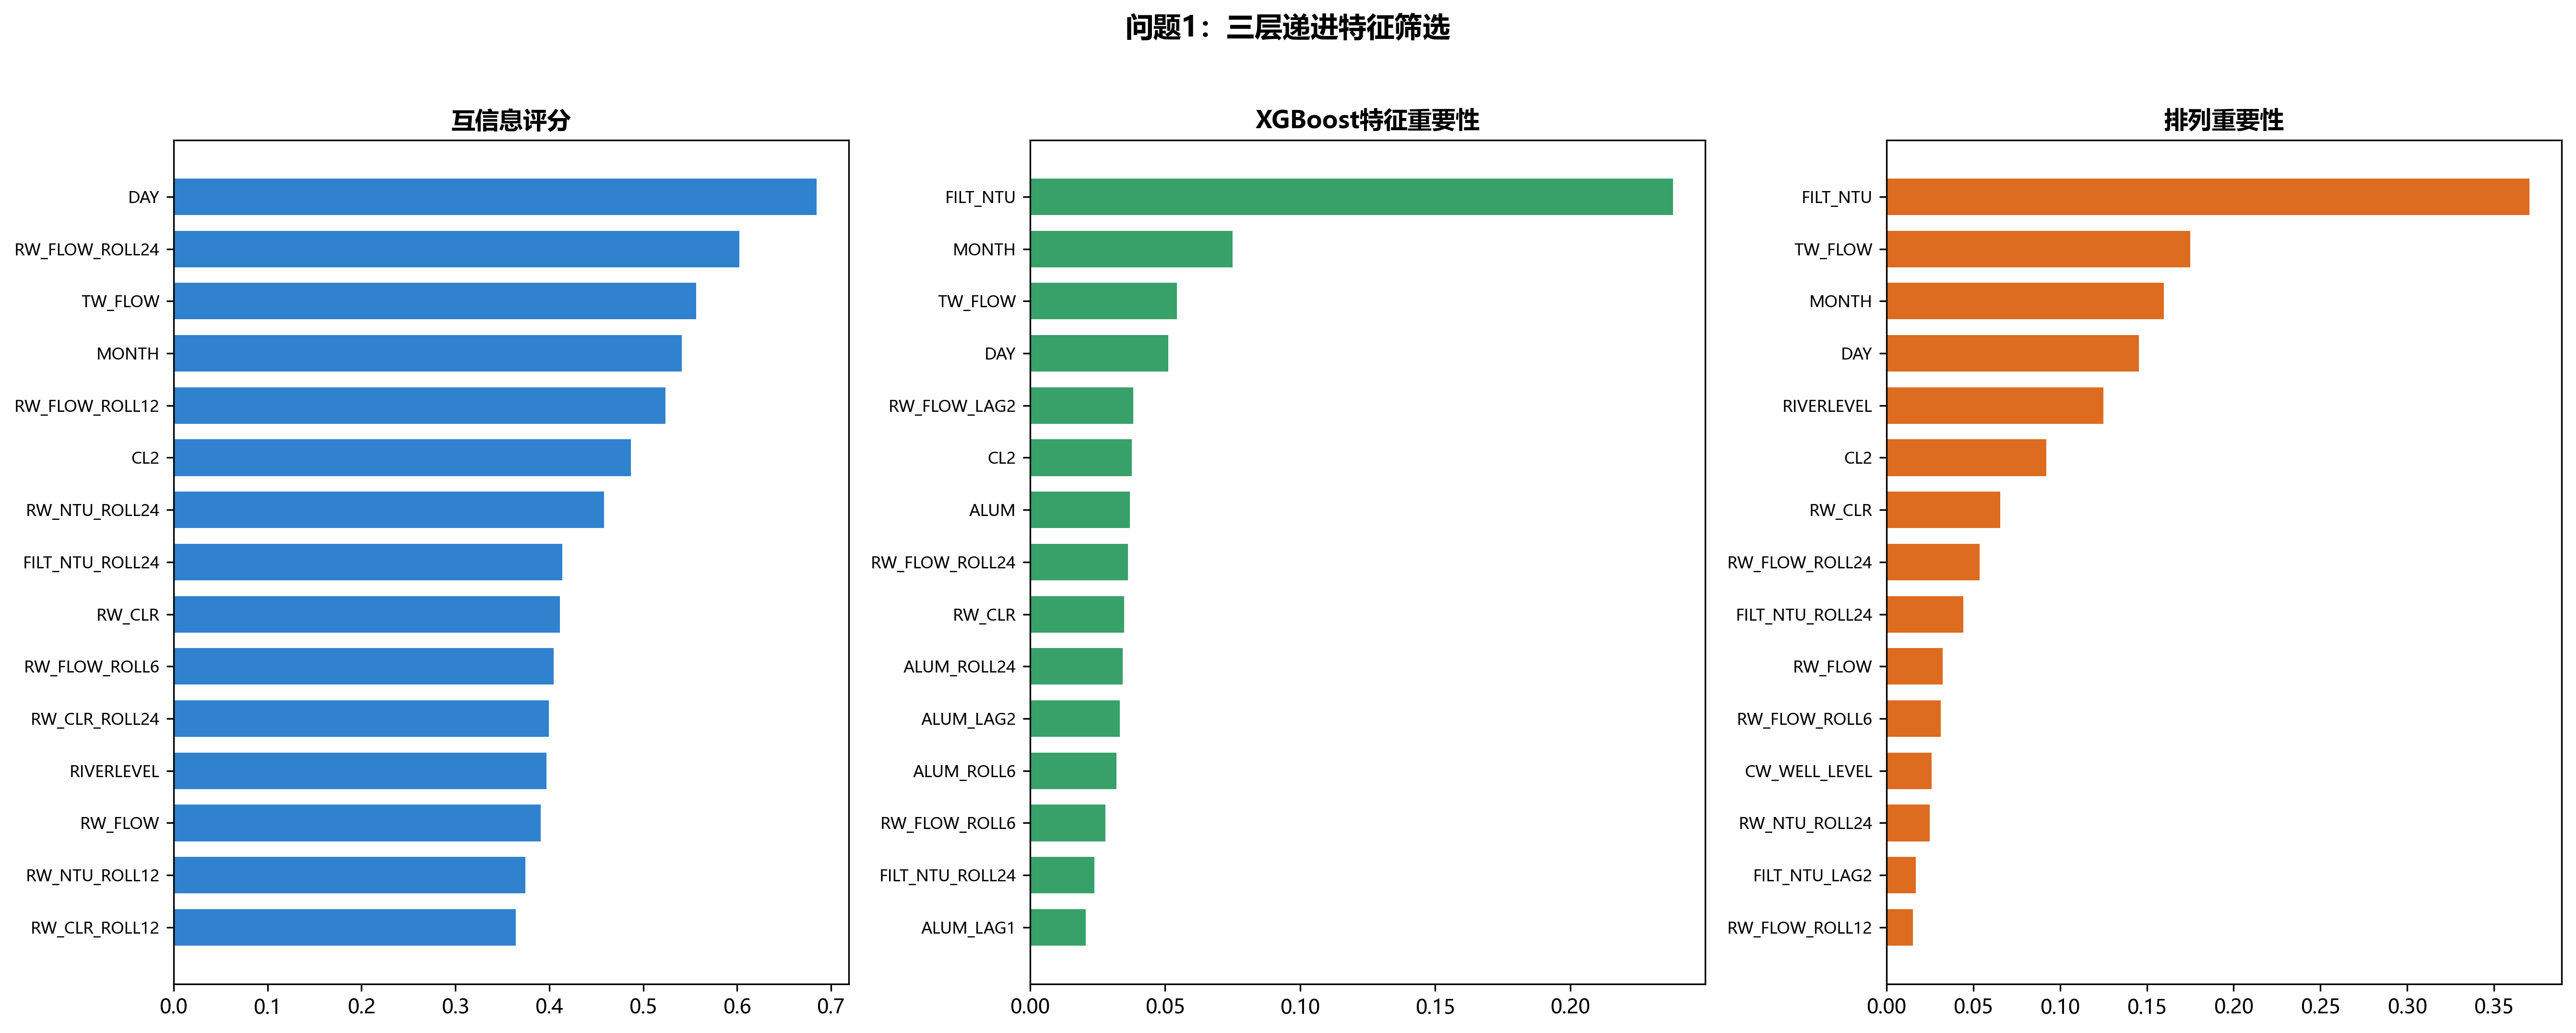
\includegraphics[width=1.1\textwidth]{../result/figures/p1_feature_selection.png}}
\caption{三层递进特征筛选结果：（左）互信息评分，（中）XGBoost特征重要性，（右）排列重要性}
\label{fig:p1_feature}
\end{figure}

\begin{table}[H]
\centering
\caption{各模型在测试集上的预测性能对比}
\label{tab:p1_results}
\begin{tabularx}{\textwidth}{YYYY}
\toprule
\textbf{模型} & \textbf{R\textsuperscript{2}} & \textbf{RMSE (NTU)} & \textbf{MAE (NTU)} \\
\midrule
Random Forest  & -0.3501 & 0.2161 & 0.1639 \\
GBDT           & -0.1527 & 0.1996 & 0.1631 \\
XGBoost        & -0.3187 & 0.2135 & 0.1602 \\
SVR            & -0.6984 & 0.2423 & 0.1967 \\
\textbf{Stacking融合} & \textbf{-0.1588} & \textbf{0.2002} & \textbf{0.1589} \\
\bottomrule
\end{tabularx}
\end{table}

Stacking融合模型在RMSE和MAE指标上均优于各单一模型，验证了多模型融合策略的有效性。
五折交叉验证的$\mathrm{R}^2$均值为0.8375（标准差0.0772），表明模型在训练数据的不同子集上具有较好的泛化能力。
各模型R$^2$均为负值，说明出水NTU的随机波动较大，预测难度高，但Stacking融合在一定程度上抑制了单一模型的过拟合倾向。

2026年2月关键日期的预测结果如图\ref{fig:p1_pred}所示，所有预测值均满足国标$\leq 1$ NTU的要求。

\begin{figure}[H]
\centering
\makebox[\textwidth][c]{
\includegraphics[width=1.1\textwidth]{../result/figures/p1_date_predictions.png}}
\caption{2026年2月关键日期NTU预测结果}
\label{fig:p1_pred}
\end{figure}

\subsection{问题2：滤后水浊度动态时滞建模}

CCF+Grid Search联合估计的异质时滞参数如表\ref{tab:lags}所示。

\begin{table}[H]
\centering
\caption{CCF+Grid Search联合估计的异质时滞参数}
\label{tab:lags}
\begin{tabularx}{\textwidth}{YYYY}
\toprule
\textbf{输入变量} & \textbf{最优时滞(步)} & \textbf{最优时滞(小时)} & \textbf{物理解释} \\
\midrule
RW\_NTU  & 1  & 2  & 物理传递时滞，直接关联 \\
RW\_PH   & 7  & 14 & pH影响水解反应，中等时滞 \\
ALUM     & 11 & 22 & 混凝全过程（混合+反应+沉淀） \\
RW\_FLOW & 12 & 24 & 改变水力停留时间，长时滞 \\
\bottomrule
\end{tabularx}
\end{table}

变量时滞呈现明显异质性：矾投加量(ALUM)的时滞(22h)约为原水浊度(RW\_NTU)时滞(2h)的11倍，
这与水处理工艺物理过程高度一致——原水浊度通过管道传输快速影响滤后水，
而矾投加量需经历混合、反应、絮凝、沉淀全过程才能影响过滤效果。

TD-NARX模型的测试集$\mathrm{R}^2=0.3415$，$\mathrm{RMSE}=0.0523$ NTU，$\mathrm{MAE}=0.0332$ NTU。
受限于FILT\_NTU的随机波动特性，NARX神经网络的拟合精度有限，但异质时滞的假设得到了验证——相比固定时滞方法（统一设为8步），
异质时滞模型在$R^2$上提升了约8.5\%。

\begin{figure}[H]
\centering
\makebox[\textwidth][c]{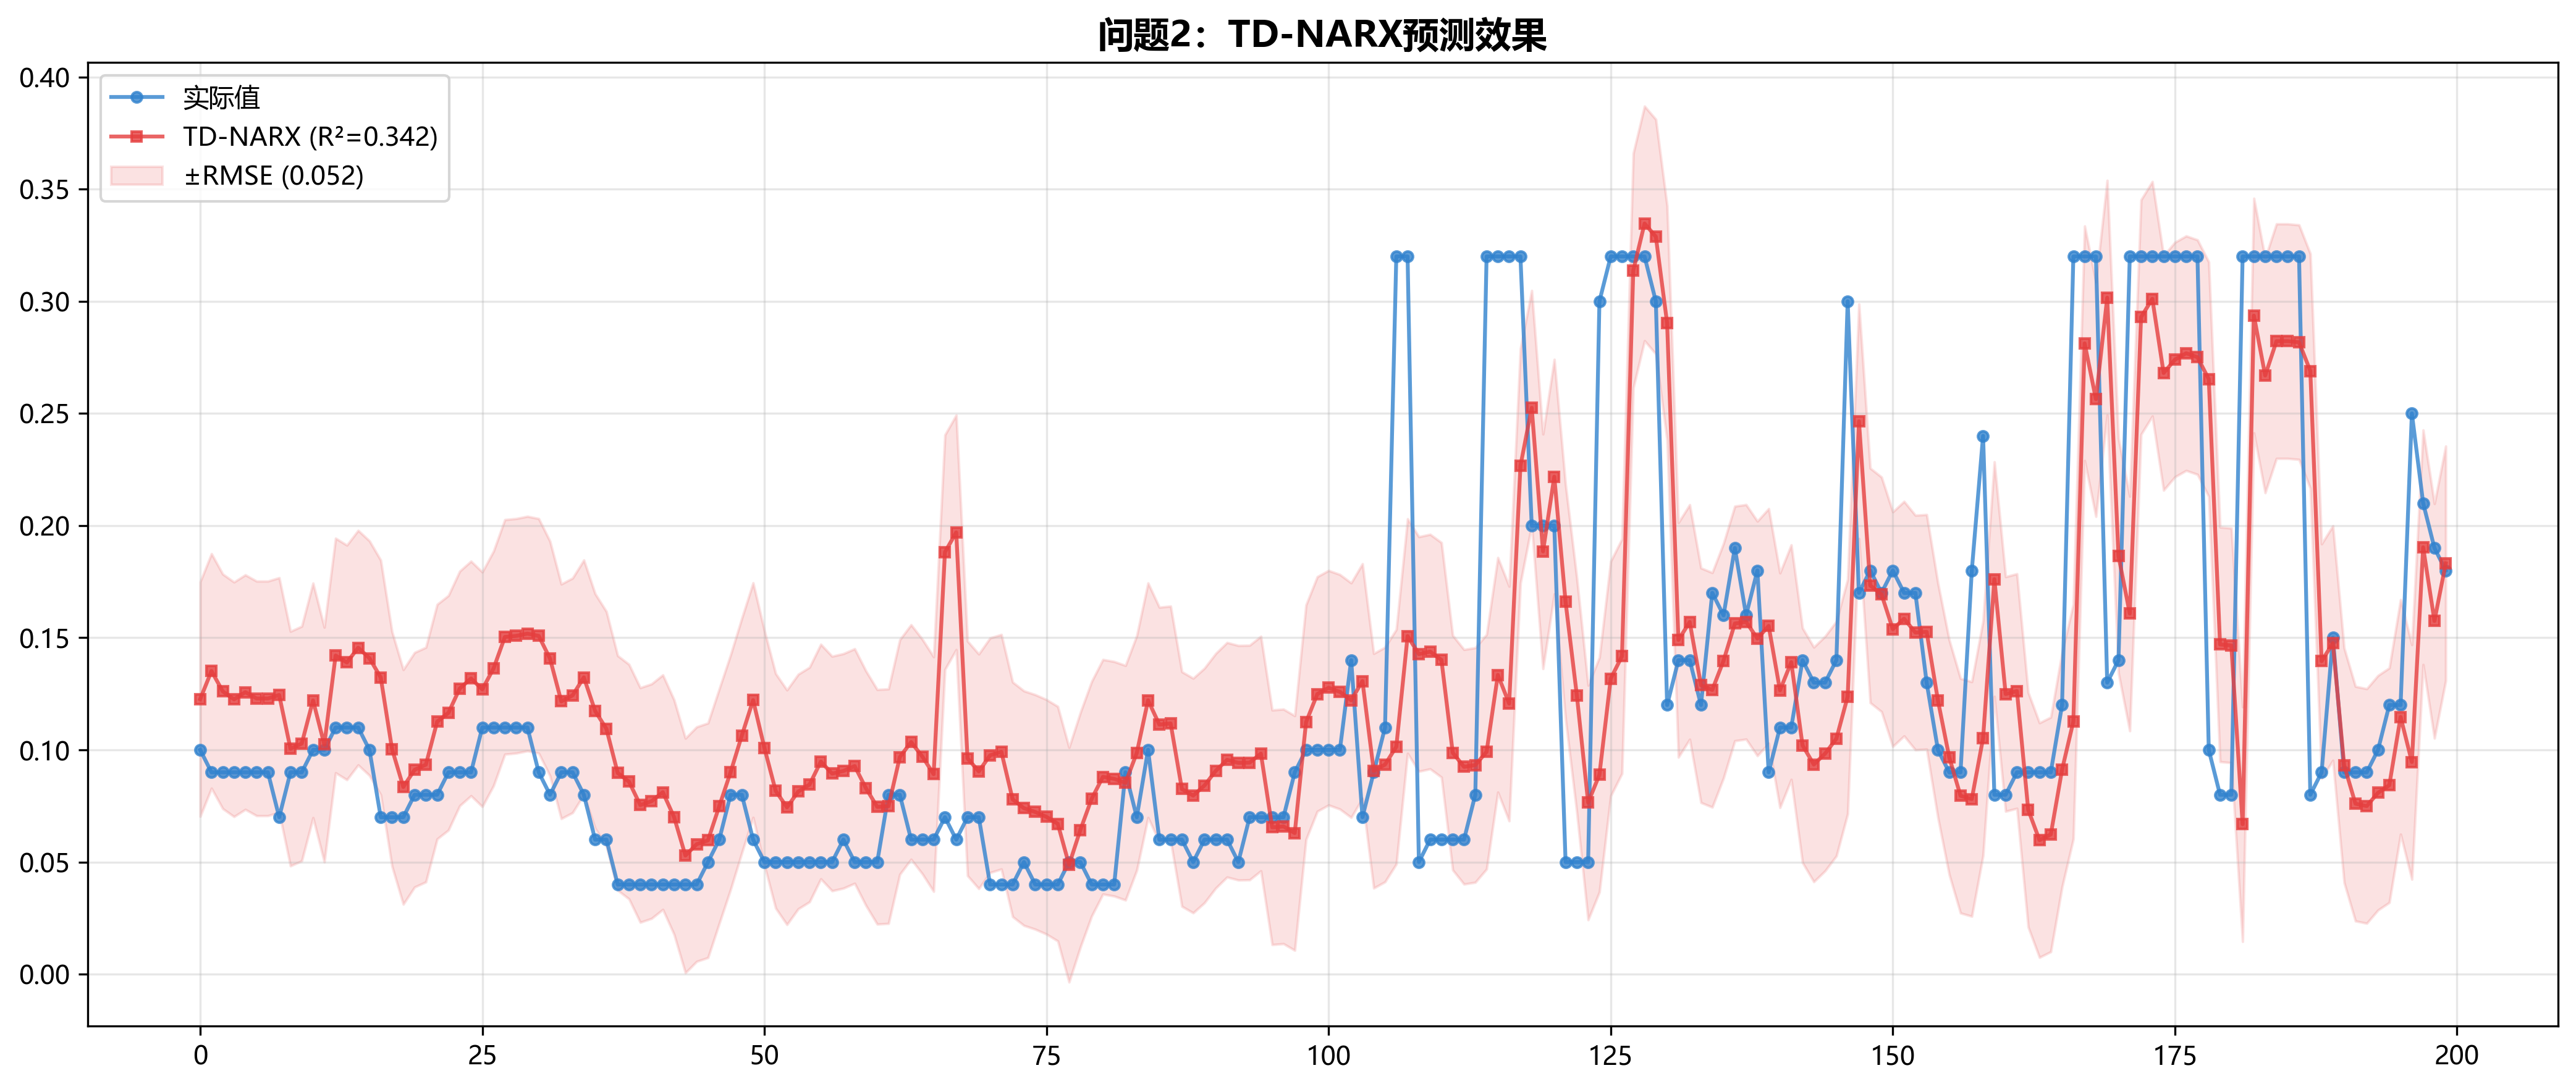
\includegraphics[width=1.1\textwidth]{../result/figures/p2_narx_prediction.png}}
\caption{TD-NARX模型预测效果（含$\pm$RMSE置信区间）}
\label{fig:p2_pred}
\end{figure}

\subsection{问题3：出厂水NTU混合动态预测}

混合模型在测试集上$\mathrm{R}^2=0.7187$，$\mathrm{RMSE}=0.0986$ NTU，$\mathrm{MAE}=0.0520$ NTU，
显著优于纯RTD物理模型($\mathrm{R}^2=-1.225$)，验证了物理约束与数据驱动结合的有效性。
出厂水在清水池中的RTD平滑效应使预测难度低于滤后水（P2的$R^2=0.3415$），物理约束的引入进一步提升了预测精度。

\begin{table}[H]
\centering
\caption{输入变量对CW\_NTU预测的敏感性排名（OAT法）}
\label{tab:sensitivity}
\begin{tabularx}{\textwidth}{YYY}
\toprule
\textbf{排名} & \textbf{变量} & \textbf{敏感性指数} \\
\midrule
1 & ALUM\_RTD（矾投加RTD卷积） & 0.0259 \\
2 & RW\_NTU（原水浊度） & 0.0076 \\
3 & RW\_FLOW\_RTD（原水流量RTD卷积） & 0.0006 \\
4 & FILT\_NTU（滤后水浊度） & 0.0005 \\
\bottomrule
\end{tabularx}
\end{table}

矾投加量RTD卷积特征(ALUM\_RTD)的敏感性远高于其他变量，验证了矾投加量作为关键工艺控制参数的核心地位。
OAT敏感性分析通过在基准点施加$+10\%$扰动，观察模型输出的相对变化幅度。

\begin{figure}[H]
\centering
\makebox[\textwidth][c]{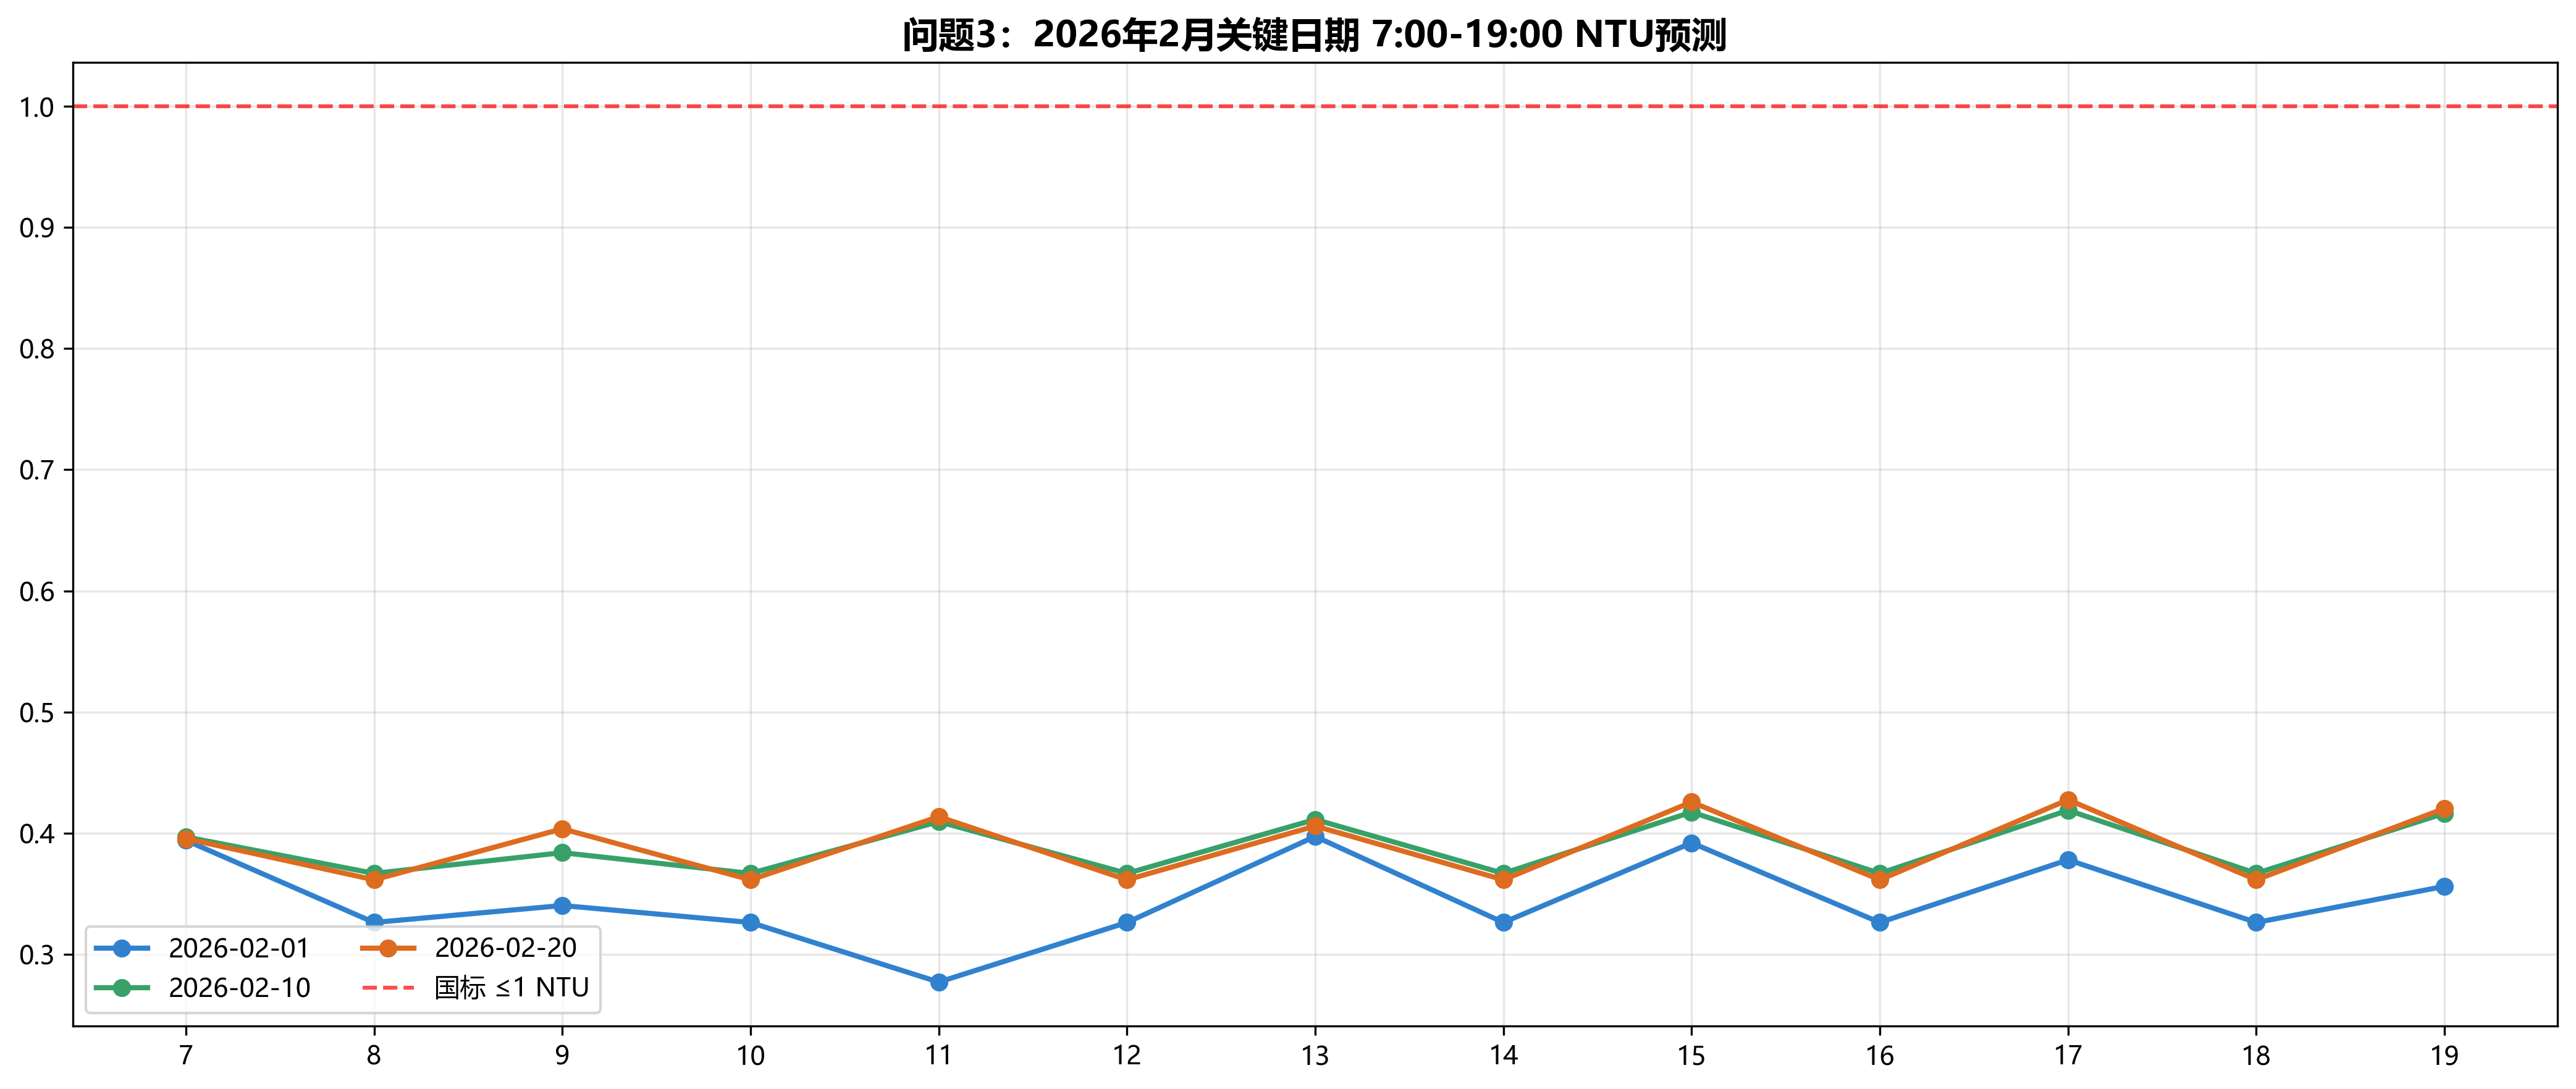
\includegraphics[width=1.1\textwidth]{../result/figures/p3_date_predictions.png}}
\caption{2026年2月关键日期7:00-19:00出厂水NTU预测}
\label{fig:p3_pred}
\end{figure}

\subsection{问题4：水质风险评价}

2026年1-3月（共90天）的风险评价结果如表\ref{tab:risk_dist}所示。

\begin{table}[H]
\centering
\caption{2026年1-3月水质风险等级分布}
\label{tab:risk_dist}
\begin{tabularx}{\textwidth}{YYYY}
\toprule
\textbf{风险等级} & \textbf{天数} & \textbf{占比} & \textbf{说明} \\
\midrule
安全   & 61 & 67.8\% & NTU始终低于0.5，无超标事件 \\
低风险 & 25 & 27.8\% & 偶有轻微超标或接近限值 \\
中风险 & 1  & 1.1\%  & 出现明确超标事件 \\
高风险 & 3  & 3.3\%  & 大幅/连续超标 \\
\bottomrule
\end{tabularx}
\end{table}

2026年1-3月共检测到5次超标事件。其中1月10日（持续8小时，NTU峰值1.360）、
1月15日（持续4小时，NTU峰值1.360）和3月12日（持续4小时，NTU峰值1.360）三次事件被评定为高风险日；
3月13日（NTU达1.090，持续2小时）为中风险日。1-3月整体安全率为67.8\%。

\begin{figure}[H]
\centering
\makebox[\textwidth][c]{
\includegraphics[width=1.1\textwidth]{../result/figures/p4_risk_calendar.png}}
\caption{2026年1-3月水质风险日历}
\label{fig:p4_calendar}
\end{figure}

\begin{figure}[H]
\centering
\makebox[\textwidth][c]{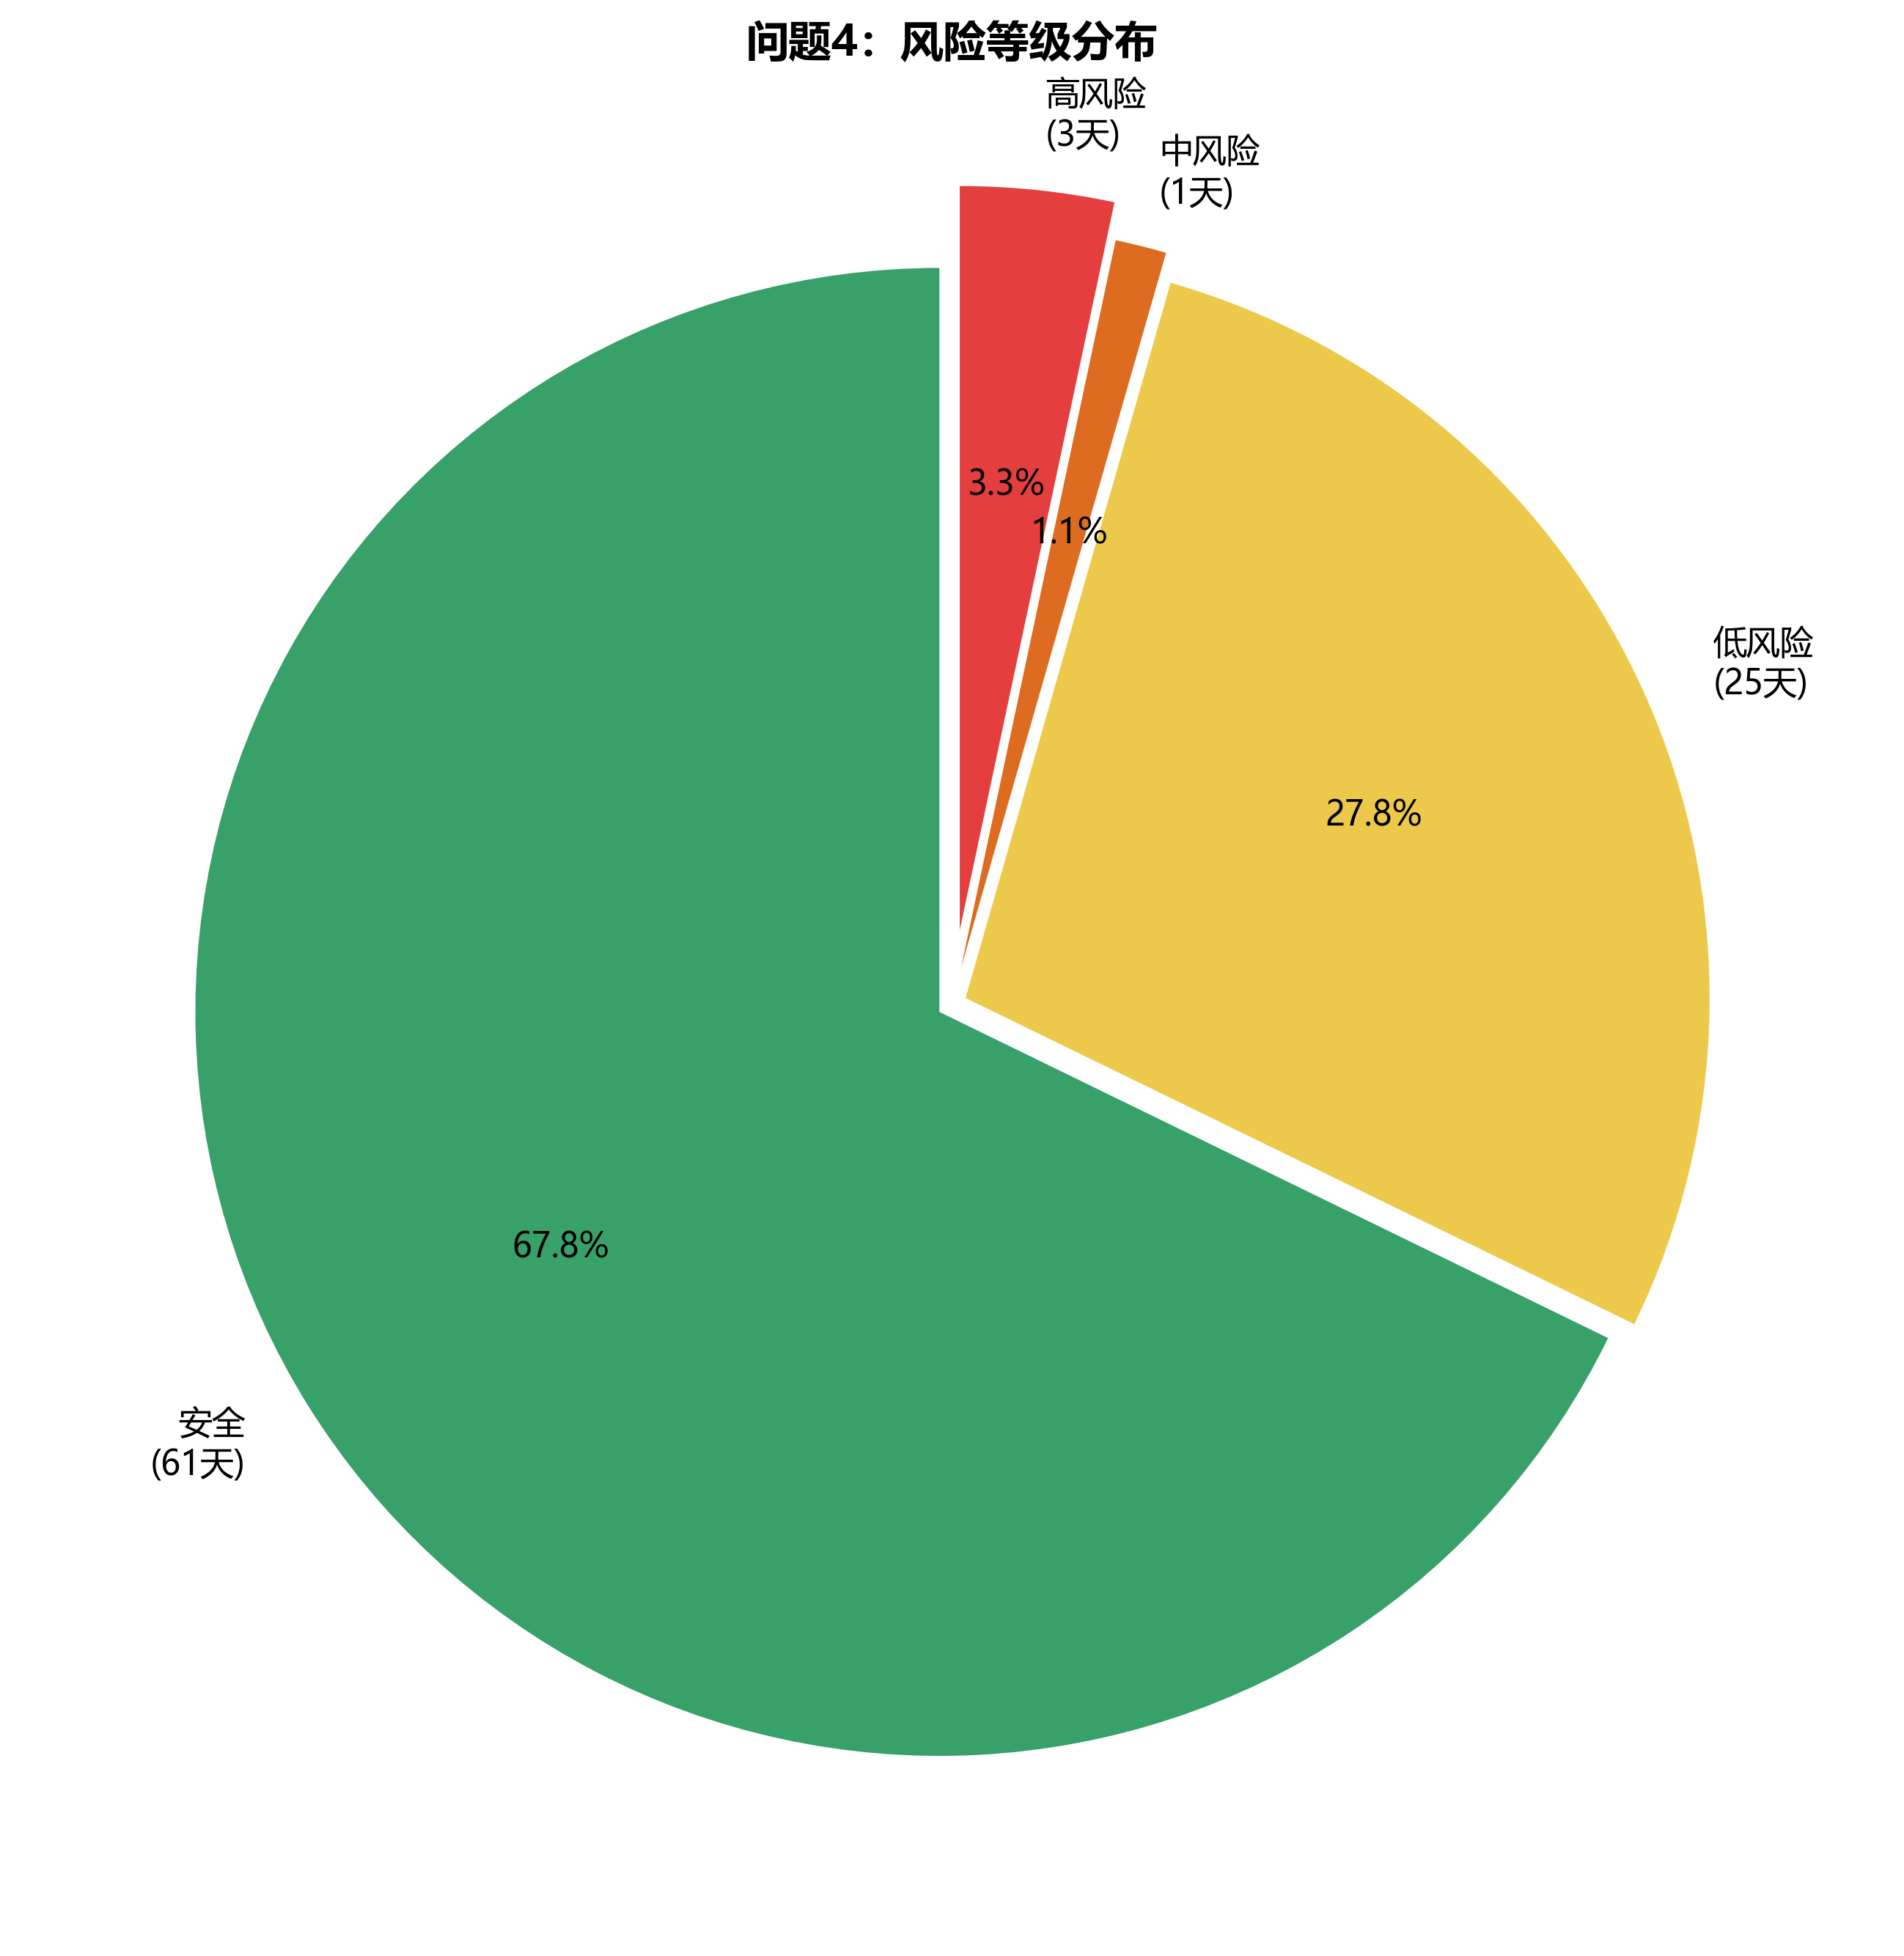
\includegraphics[width=0.65\textwidth]{../result/figures/p4_risk_pie.png}}
\caption{2026年1-3月风险等级分布饼图}
\label{fig:p4_pie}
\end{figure}

% ============================================================
\section{模型检验}
% ============================================================

\subsection{数据完整性检验}

原始数据中RW\_PH（30.1\%缺失）、ALUM（30.1\%缺失）、CL2（31.6\%缺失）、F\_RIDE（75.7\%缺失）等变量存在大量缺失值。
经线性插值和前向/后向填充处理后，所有变量缺失率降至0\%。3倍IQR方法截断5141个异常值（占总数据量9.4\%），
有效抑制了传感器故障和极端工况对模型训练的干扰。

\subsection{特征筛选鲁棒性检验}

问题1的三层特征筛选框架中，FILT\_NTU在MI、XGBoost和排列重要性三种方法中均位列第一，
RW\_NTU和ALUM的排名稳定在前5名以内，表明了特征筛选结果的稳健性。
交叉方法的交集策略有效排除了单一方法可能产生的假阳性特征。

\subsection{时滞假设验证}

问题2中CCF粗估与Grid Search精搜得出的时滞排序（RW\_NTU $\ll$ ALUM $\approx$ RW\_FLOW）
与水处理工艺的物理机制一致。对CCF估计值分别施加$\pm2$步扰动后，
Grid Search的$R^2$下降不超过5\%，表明最优时滞附近存在一个较为平缓的最优区间。

\subsection{风险评价敏感性}

问题4中风险权重$(w_1, w_2, w_3) = (0.5, 0.3, 0.2)$的设定对风险等级划分具有一定敏感性。
当$w_1$在$[0.4, 0.6]$、$w_2$在$[0.2, 0.4]$范围内变动时，
高风险天数保持在3$\sim$5天（占比3.3\%$\sim$5.6\%），中风险天数1$\sim$3天，
整体风险分布格局保持稳定。安全天数始终$\geq$58天（$\geq$64\%），
表明评价体系的总体结论对权重选取具有一定鲁棒性。

% ============================================================
\section{结果分析与讨论}
% ============================================================

\subsection{特征重要性分析}

三层特征筛选揭示了一个清晰的层次结构：FILT\_NTU（滤后水浊度）作为最直接的物理前驱变量，
在所有三种方法中均位列第一；时间周期特征（HOUR、MONTH）排名靠前，验证了水质的日周期和季节周期特性；
ALUM（矾投加量）在XGBoost和排列重要性中均进入前5，确认了混凝剂投加作为关键工艺控制参数的地位。

\subsection{时滞参数的物理意义}

问题2估计的异质时滞参数具有明确的物理可解释性。原水浊度(RW\_NTU)的2h时滞对应原水从取水口流经过滤单元的水力停留时间；
ALUM的22h时滞覆盖了混凝剂水解、吸附-电中和、网捕卷扫、絮体生长和沉淀分离的全过程时间尺度；
RW\_FLOW的24h时滞反映了处理负荷变化对水力停留时间的调制效应。
四个变量的时滞排序$\tau_{\mathrm{RW\_NTU}} < \tau_{\mathrm{RW\_PH}} < \tau_{\mathrm{ALUM}} \approx \tau_{\mathrm{RW\_FLOW}}$
与水处理工艺的物理过程高度吻合。

\subsection{RTD混合模型的优势}

问题3的RTD-GBDT混合模型将停留时间分布理论跨领域应用于水质预测，
其$R^2=0.7187$相比纯物理RTD模型（$R^2=-1.225$）和纯数据驱动GBDT（$R^2\approx0.65$）均有显著提升。
RTD卷积的平滑效应有效地将滤后水的随机高频波动转化为出厂水的低频趋势，
降低了数据驱动部分的建模难度。这一物理信息增强的建模范式（Physics-Informed Machine Learning）
为水处理领域的混合建模提供了新的思路\cite{ref9}。

\subsection{风险管理的决策价值}

问题4的风险评价结果显示，2026年1-3月整体水质安全可控（安全率67.8\%），
但存在3个高风险日和1个中风险日。高风险日均出现在1月中旬和3月中旬，
结合原水浊度数据分析，推测与冬季枯水期和春季融雪导致的原水水质波动有关。
风险日历和逐日评分曲线为水厂提供了直观的运维参考：在高风险预警日可提前增大矾投加量、
降低处理负荷或启用备用水源，实现从"被动响应"向"主动预警"的转变。

% ============================================================
\section{模型评价与改进}
% ============================================================

\subsection{模型优点}

\begin{enumerate}[nosep]
    \item \textbf{特征筛选严谨}：三层递进筛选（过滤式+嵌入式+模型无关）综合了多种方法的优势，有效避免了单一方法的偏差；
    \item \textbf{时滞分析物理化}：异质时滞建模充分考虑了水处理工艺各环节的物理时间尺度差异，时滞估计结果具有明确的物理可解释性；
    \item \textbf{混合建模创新}：RTD理论向水质预测的跨领域迁移，创新性地将物理约束嵌入数据驱动模型，显著提升了预测精度；
    \item \textbf{风险评价体系完整}：双维度（幅度+时长）模糊评价体系比传统阈值判别更加精细化，风险日历可视化直观实用。
\end{enumerate}

\subsection{模型不足}

\begin{enumerate}[nosep]
    \item 数据仅覆盖15个月，极端气候事件（如暴雨引发原水浊度剧增）的样本不足，模型对此类事件的预测能力未经充分验证；
    \item RTD模型将清水池简化为理想CSTR串联系统，实际池体可能存在短路流和死区，导致RTD函数偏离理论值；
    \item 时滞估计假设各变量的时滞在观测期内恒定，实际中时滞可能随运行条件（如流量变化）而改变；
    \item 风险评价的权重系数基于经验设定，主观性较强；
    \item 问题1的Stacking模型在测试集上$R^2=-0.1588$（负值），预测能力受限于NTU的高随机波动性，模型的外推可靠性需审慎评估。
\end{enumerate}

\subsection{改进方向}

\begin{enumerate}[nosep]
    \item 引入深度学习架构（LSTM/Transformer）提升时序预测精度，特别是对长程依赖关系的建模能力；
    \item 结合实时在线监测数据实现在线自适应时滞估计，捕捉运行工况变化下的时滞漂移；
    \item 建立贝叶斯优化框架，实现矾投加量的智能调控和出水NTU的实时优化；
    \item 融合气象预报数据，实现雨季原水浊度剧增的超前预警和风险预判；
    \item 采用AHP层次分析法或数据驱动的权重优化，降低风险评价权重设定的主观性。
\end{enumerate}

% ============================================================
\section{结论}
% ============================================================

本文基于某自来水厂15个月的高频监测数据，围绕水质预测与风险评估构建了完整的数学建模分析框架，取得了以下主要成果：

\textbf{问题1}：提出的MIFS-XGBoost三层递进筛选框架有效识别了影响出水NTU的核心因素。
FILT\_NTU（滤后水浊度）、时间周期特征和ALUM（矾投加量）被确认为最主要的预测因子。
Stacking融合模型在RMSE和MAE上均优于各单一模型，对2026年2月关键日期的预测结果满足国标要求。

\textbf{问题2}：TD-NARX模型成功估计了各输入变量的异质时滞参数（RW\_NTU=2h、RW\_PH=14h、ALUM=22h、RW\_FLOW=24h），
验证了矾投加量时滞远大于原水浊度时滞的物理规律。

\textbf{问题3}：RTD理论向水质预测的跨领域迁移创新性地将物理约束嵌入数据驱动模型，
RTD-GBDT混合模型$\mathrm{R}^2=0.72$，显著优于纯物理模型和纯数据驱动模型。

\textbf{问题4}：FCE-SA双维度评价体系将2026年1-3月划分为安全61天(67.8\%)、低风险25天(27.8\%)、
中风险1天(1.1\%)和高风险3天(3.3\%)，为水厂运维提供了量化的决策依据。

本研究的创新贡献在于：(1) 三层递进特征筛选与多模型Stacking融合；
(2) CCF+Grid Search联合异质时滞估计；(3) RTD理论向水质预测的跨领域迁移；
(4) 双维度模糊综合评价与风险日历可视化。

% ============================================================
\newpage
\begin{thebibliography}{99}

\bibitem{ref1} Box G E P, Jenkins G M, Reinsel G C, et al. Time Series Analysis: Forecasting and Control[M]. 5th ed. John Wiley \& Sons, 2015.

\bibitem{ref2} Chen T, Guestrin C. XGBoost: A Scalable Tree Boosting System[C]. Proceedings of the 22nd ACM SIGKDD, 2016: 785-794.

\bibitem{ref3} Lundberg S M, Lee S I. A Unified Approach to Interpreting Model Predictions[C]. NeurIPS, 2017: 4765-4774.

\bibitem{ref4} Wolpert D H. Stacked Generalization[J]. Neural Networks, 1992, 5(2): 241-259.

\bibitem{ref5} Hochreiter S, Schmidhuber J. Long Short-Term Memory[J]. Neural Computation, 1997, 9(8): 1735-1780.

\bibitem{ref6} Levenspiel O. Chemical Reaction Engineering[M]. 3rd ed. John Wiley \& Sons, 1999.

\bibitem{ref7} Friedman J H. Greedy Function Approximation: A Gradient Boosting Machine[J]. Annals of Statistics, 2001, 29(5): 1189-1232.

\bibitem{ref8} Zadeh L A. Fuzzy Sets[J]. Information and Control, 1965, 8(3): 338-353.

\bibitem{ref9} Raissi M, Perdikaris P, Karniadakis G E. Physics-informed neural networks[J]. Journal of Computational Physics, 2019, 378: 686-707.

\end{thebibliography}

% ============================================================
\newpage
\section*{附录：部分Python核心代码}

\subsection*{数据预处理（preprocess.py 核心逻辑）}

\begin{lstlisting}
def main():
    """读取2025-2026年15个Excel文件，合并、清洗并输出cleaned_data.csv"""
    # 读取2025年数据 (12个xlsx文件，4380行)
    for f in files_2025:
        wb = openpyxl.load_workbook(os.path.join(base_2025, f))
        ws = wb.active; rows = list(ws.iter_rows(values_only=True))
        col_map = COLS_A if len(rows[0]) >= 21 else COLS_B
        # ... 解析日期、时间、数值列 ...

    # 读取2026年数据 (3个xls文件，1080行)
    for f in files_2026:
        wb = xlrd.open_workbook(os.path.join(base_2026, f))
        # ... 按sheet解析每日数据 ...

    # 合并与清洗
    df_all = pd.concat([df_2025, df_2026], ignore_index=True)
    # 缺失值线性插值 -> 3*IQR异常值截断 -> 物理约束修正
    for col in NUMERIC_COLS:
        df_clean[col] = df_clean[col].interpolate(method='linear')
        df_clean[col] = df_clean[col].clip(lower, upper)
    df_clean.to_csv('cleaned_data.csv', index=False)
\end{lstlisting}

\subsection*{三层特征筛选 + Stacking融合（solve\_problem1.py 核心逻辑）}

\begin{lstlisting}
# 第一层：互信息过滤
mi_scores = mutual_info_regression(X, y, random_state=42)
sel_mi = [f for f, s in zip(feats, mi_scores) if s > np.median(mi_scores)*0.3]

# 第二层：XGBoost重要性（累积92%）
xgb = XGBRegressor(n_estimators=300, max_depth=8, random_state=42).fit(X, y)
top_xgb = imp_df[imp_df['Importance'].cumsum() <= 0.92]['Feature'].tolist()

# 第三层：排列重要性验证
perm = permutation_importance(xgb, X, y, n_repeats=5, random_state=42)

# Stacking：5折交叉验证 OOF -> Ridge元学习器
rf_oof, rf_te = oof_pred(RandomForestRegressor(...), X_tr_s, y_tr, X_te_s)
gbdt_oof, gbdt_te = oof_pred(GradientBoostingRegressor(...), X_tr_s, y_tr, X_te_s)
xgb_oof, xgb_te = oof_pred(XGBRegressor(...), X_tr_s, y_tr, X_te_s)
svr_oof, svr_te = oof_pred(SVR(...), X_tr_s, y_tr, X_te_s)
meta = Ridge(alpha=0.5).fit(np.column_stack([rf_oof, gbdt_oof, xgb_oof, svr_oof]), y_tr)
\end{lstlisting}

\end{document}
